\documentclass{article}
\usepackage{fullpage}
\usepackage{color}
\usepackage[normalem]{ulem}
\usepackage{hyperref}
\hypersetup{colorlinks}
\newcommand{\eric}{\textcolor{blue}{[Eric]}}
\newcommand{\richard}{\textcolor{red}{[Richard]}}
\newcommand{\taylor}{\textcolor{green}{[Taylor]}}
\newcommand{\susi}{\textcolor{cyan}{[Susi]}}
\hyphenpenalty=100000
\usepackage{graphicx}
\DeclareGraphicsExtensions{.pdf,.png,.jpg}
\begin{document}
\setlength{\voffset}{3.5in}
\title{Milestone 5}
\author{Team Sriram / Team 15\\
(Susi Cisneros, Eric Henderson, Taylor Purviance and Richard Thai)}
\date{10 February 2012}
\maketitle
\clearpage
\setlength{\voffset}{0pt}
\tableofcontents
\clearpage
~\\
\begin{Large}\textbf{Changes (based off Git commits)}\end{Large}\\
~\\
\begin{tabular}{ | p{2in} | p{4.5in} | }
\hline
\textbf{Date Time} & \textbf{Description}\\
\hline
\hline
9 February 2012 11:10 am & Initial Milestone 5 created\\
\hline
\end{tabular}

\clearpage

\section{Introduction}
This document is intended to extend the fourth milestone, which defined the nine GRASP principles and explained their application (or intended application) to the project as well as why they were preferred over any other proposed solution.  In addition, the fourth milestone also explored the tests that were used to drive and develop the system (test-driven-development approach).  This document serves as a compilation of all of our previous work, including some corrections to design flaws and erratum which existed in previous milestones.  This document also discusses the application of Gang of Four and GRASP principles to the final project deliverable.\\

\section{Domain Model}
\subsection{Legend}
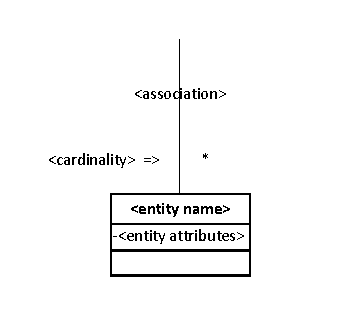
\includegraphics[keepaspectratio, width=6in]{domain_model_legend.pdf}\\
\subsection{Diagram}
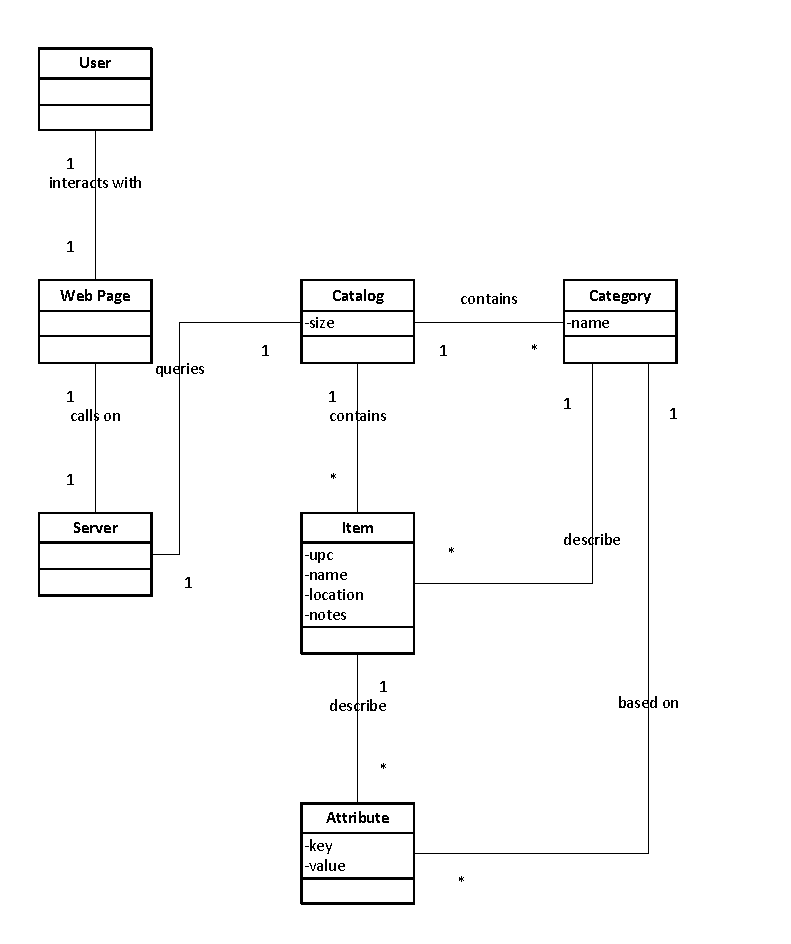
\includegraphics[keepaspectratio, width=6in]{domain_model.pdf}\\

\section{System Sequence Diagrams}
The system sequence diagrams show how the user and the system interact during the main operations of the system.\\
\subsection{Legend}
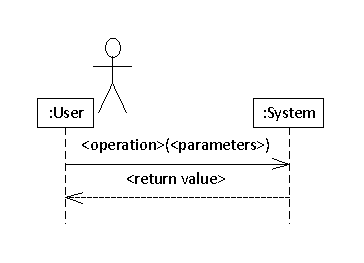
\includegraphics[keepaspectratio, width=6in]{ssd_legend.pdf}\\
\subsection{Add Item}
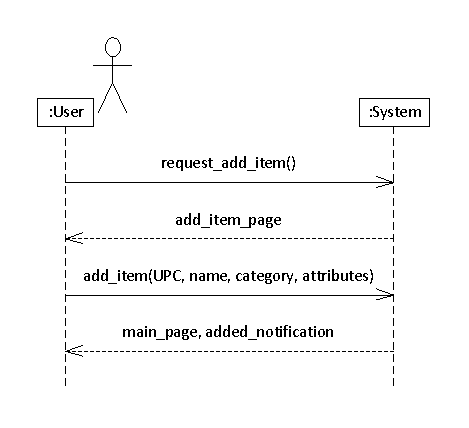
\includegraphics[keepaspectratio, width=6in]{ssd_add_item.pdf}\\
\subsection{View Item}
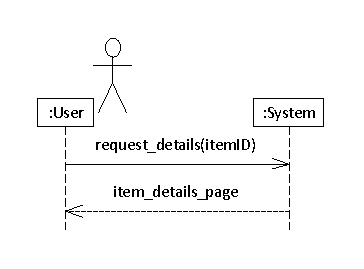
\includegraphics[keepaspectratio, width=6in]{ssd_view_item_details.pdf}\\
\subsection{Edit Item}
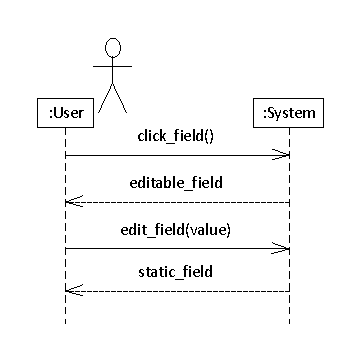
\includegraphics[keepaspectratio, width=6in]{ssd_edit_item_details.pdf}\\
\subsection{Basic Search}
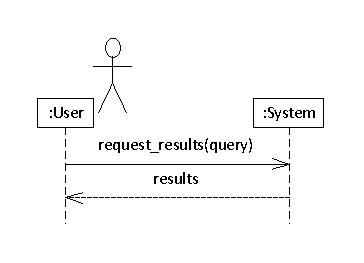
\includegraphics[keepaspectratio, width=6in]{ssd_basic_search.pdf}\\
\subsection{Advanced Search}
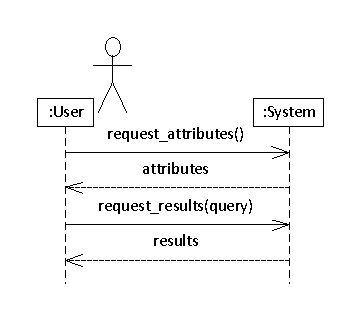
\includegraphics[keepaspectratio, width=6in]{ssd_advanced_search.pdf}\\
\subsection{Search Results Sorting}
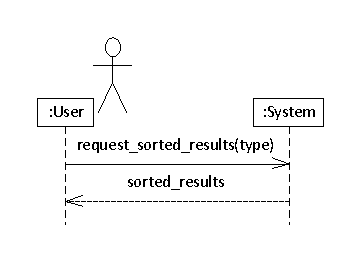
\includegraphics[keepaspectratio, width=6in]{ssd_search_result_sorting.pdf}\\
\subsection{Generate Report}
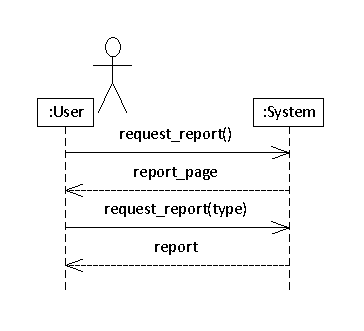
\includegraphics[keepaspectratio, width=6in]{ssd_generate_report.pdf}\\

\section{Operation Contracts}
The operation contracts show the difference between the state of the system before and after a command.  We choose to show the add item and edit field methods since the system sequence diagrams were not able to provide adequate detail for these operations.\\
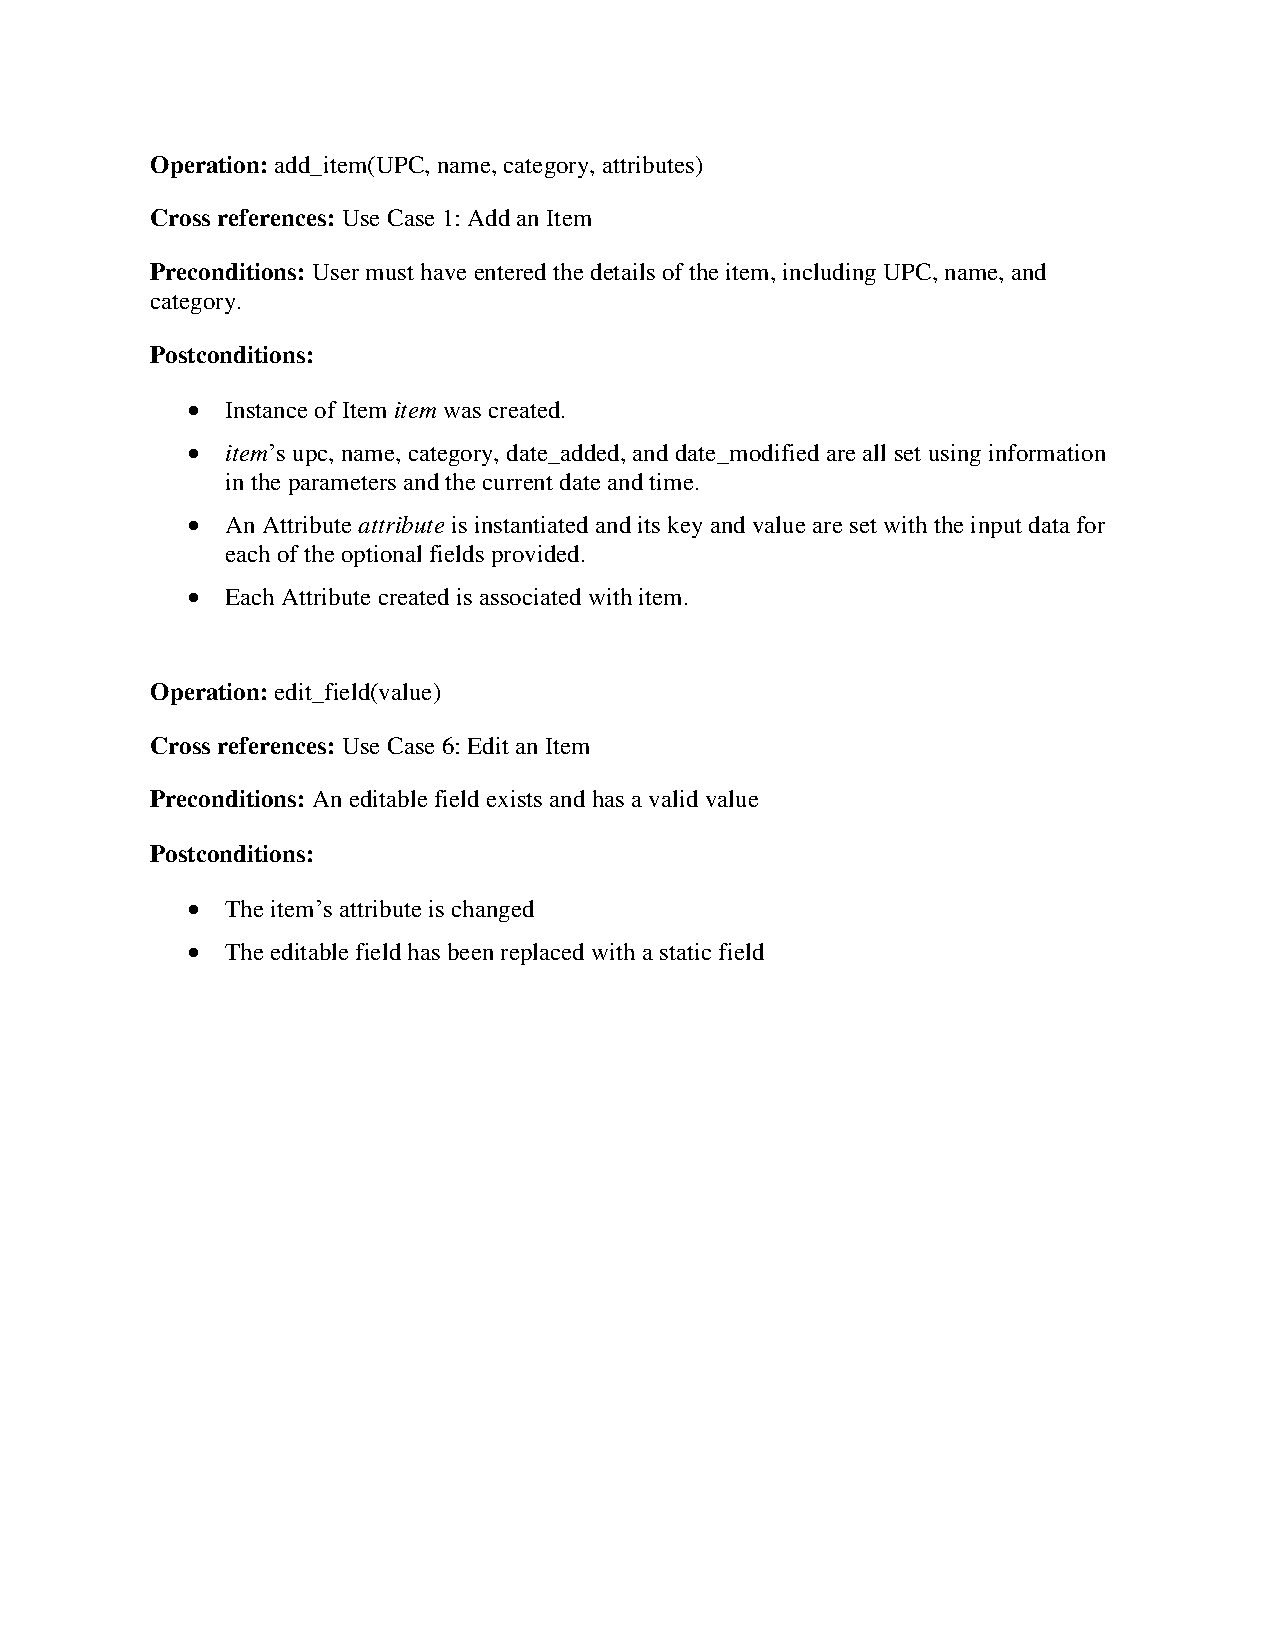
\includegraphics[keepaspectratio, width=6in]{Operational_Contracts.pdf}\\

\section{Design Class Diagram}
The design class diagram shows the relationships the classes in the system have with each other.  It also shows the attributes each class has and the operations that each class can perform.\\
\subsection{Legend}
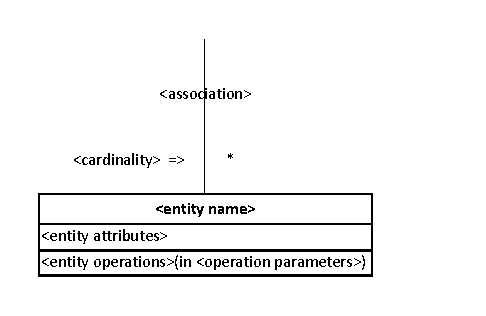
\includegraphics[keepaspectratio, width=6in]{class_diagram_legend.pdf}
\subsection{Diagram}
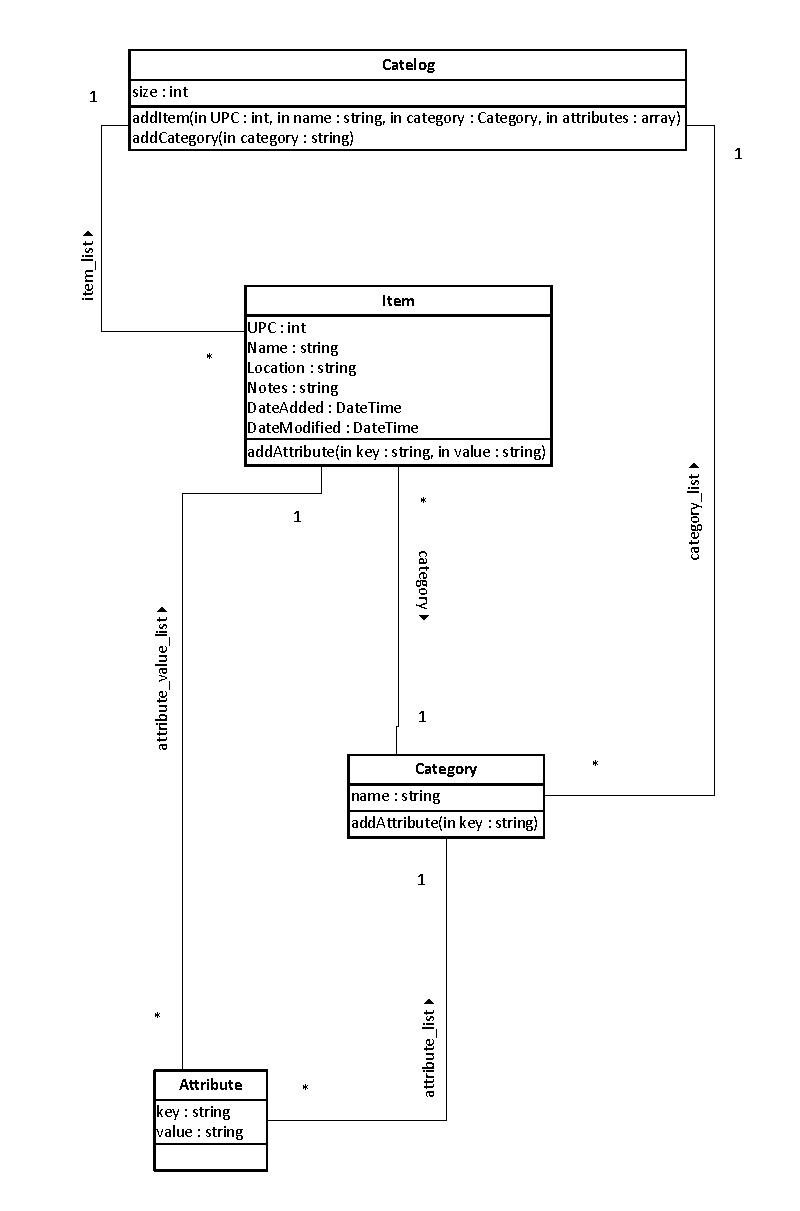
\includegraphics[keepaspectratio, width=5.25in]{class_diagram.pdf} \\

\section{Logical Architecture and Package Diagram}
This diagram shows how the main elements of the system interact with each other.  It also shows which classes are part of the same layer.  The layers represent the three major parts of the system, the user interface, the domain of the system and the technical services that the system employs. \\
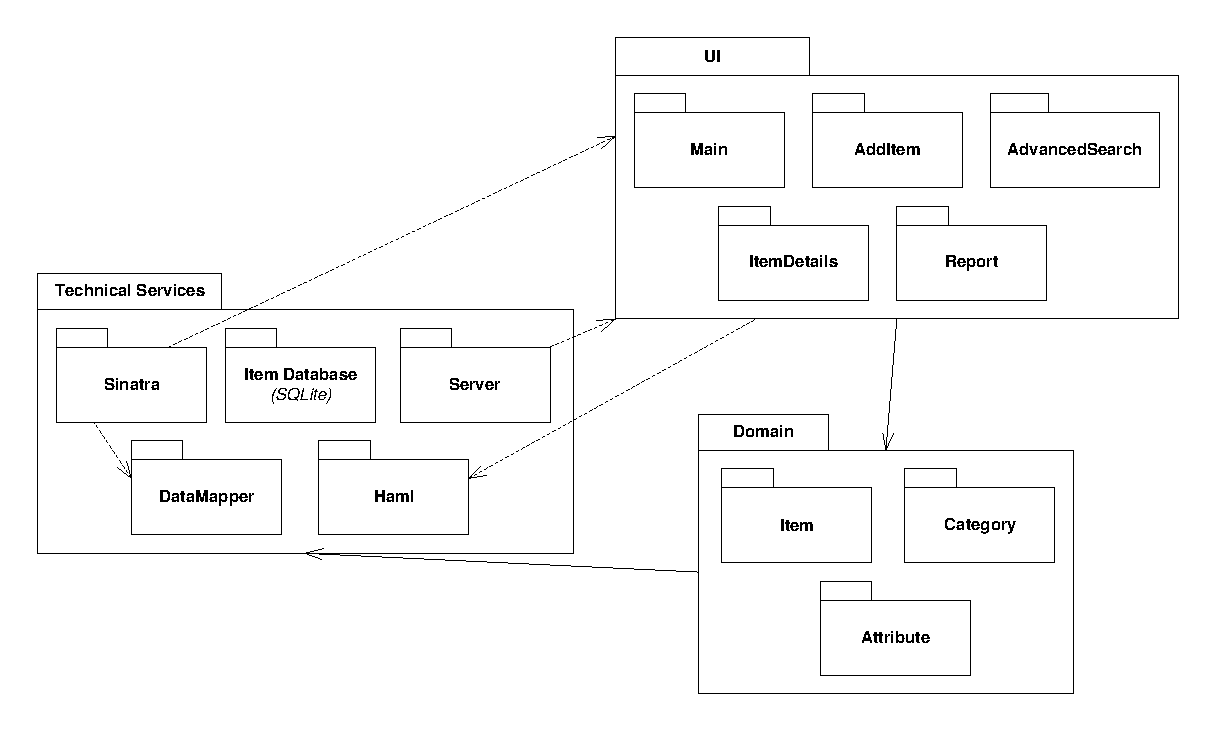
\includegraphics[keepaspectratio, width=6in]{package_diagram.pdf}\\

\section{Interaction Diagrams}
Interaction diagrams show how objects interact through messages.  For this system, we decided that sequence diagrams were more appropriate as they clearly communicate the order in which each action is performed.\\
\subsection{Sequence Diagrams}
\subsubsection{Legend}
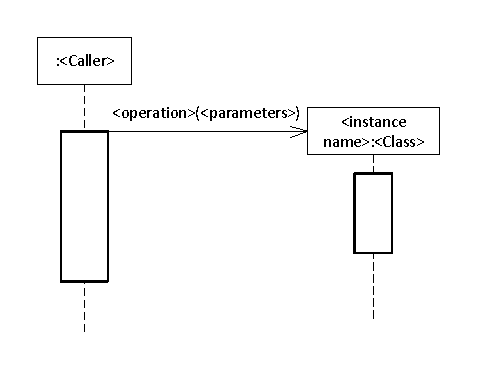
\includegraphics[keepaspectratio, width=6in]{sd_legend.pdf}\\
\subsubsection{Add Attribute to an Item}
We chose to expand this action since it will be the most frequent operation our system will do.  No matter how many items are added to the system, the action occurs repetitively with minor variations.\\
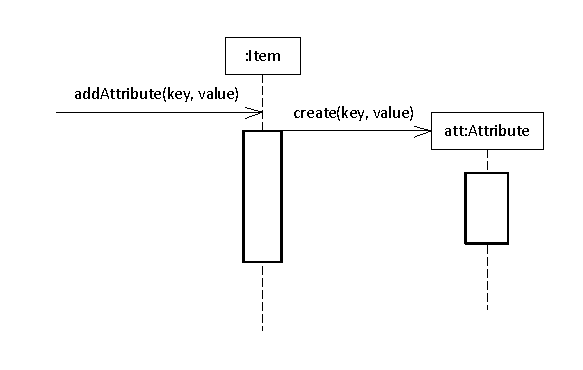
\includegraphics[keepaspectratio, width=6in]{sd_item_add_attribute.pdf}\\
\subsubsection{Add New Item}
This operation was made into an SD to show how our system handles our most important operation.  Without the ability to add items, this system would be useless.\\
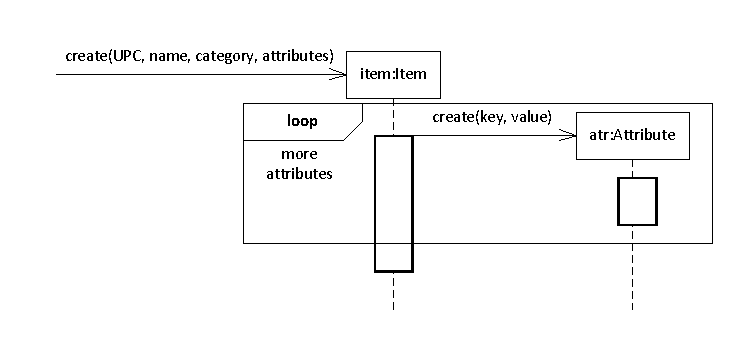
\includegraphics[keepaspectratio, width=6in]{sd_catalog_add_item.pdf}\\
\subsubsection{Add New Category}
A category is an important way for the system to differentiate the items it contains.  This is why we decided to expand this operation.\\
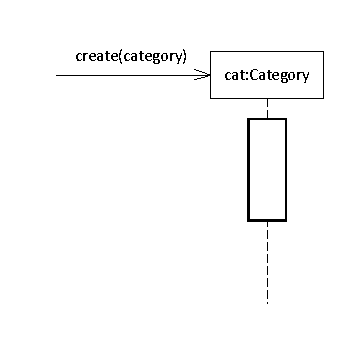
\includegraphics[keepaspectratio, width=6in]{sd_catalog_add_category.pdf}\\
\subsubsection{Add Attribute to the Category}
In order for our system to be more specific about the different items in each category, we add different attributes that are defined for the category.  This SD shows how our system handles adding new category attributes.\\
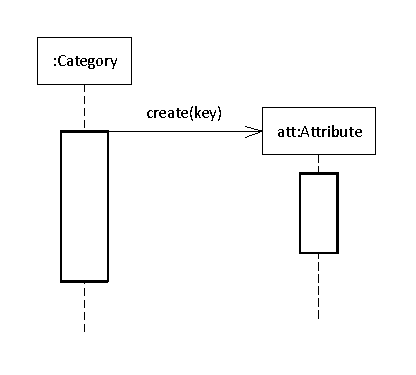
\includegraphics[keepaspectratio, width=6in]{sd_category_add_attribute.pdf}\\

\section{Activity Diagram}
\subsection{Legend}
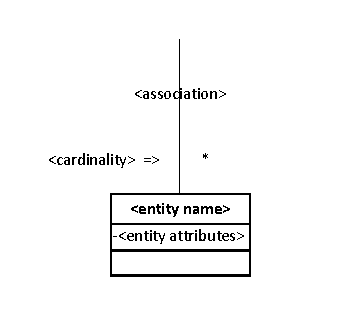
\includegraphics[keepaspectratio, width=6in]{domain_model_legend.pdf}\\
\subsection{Diagram}
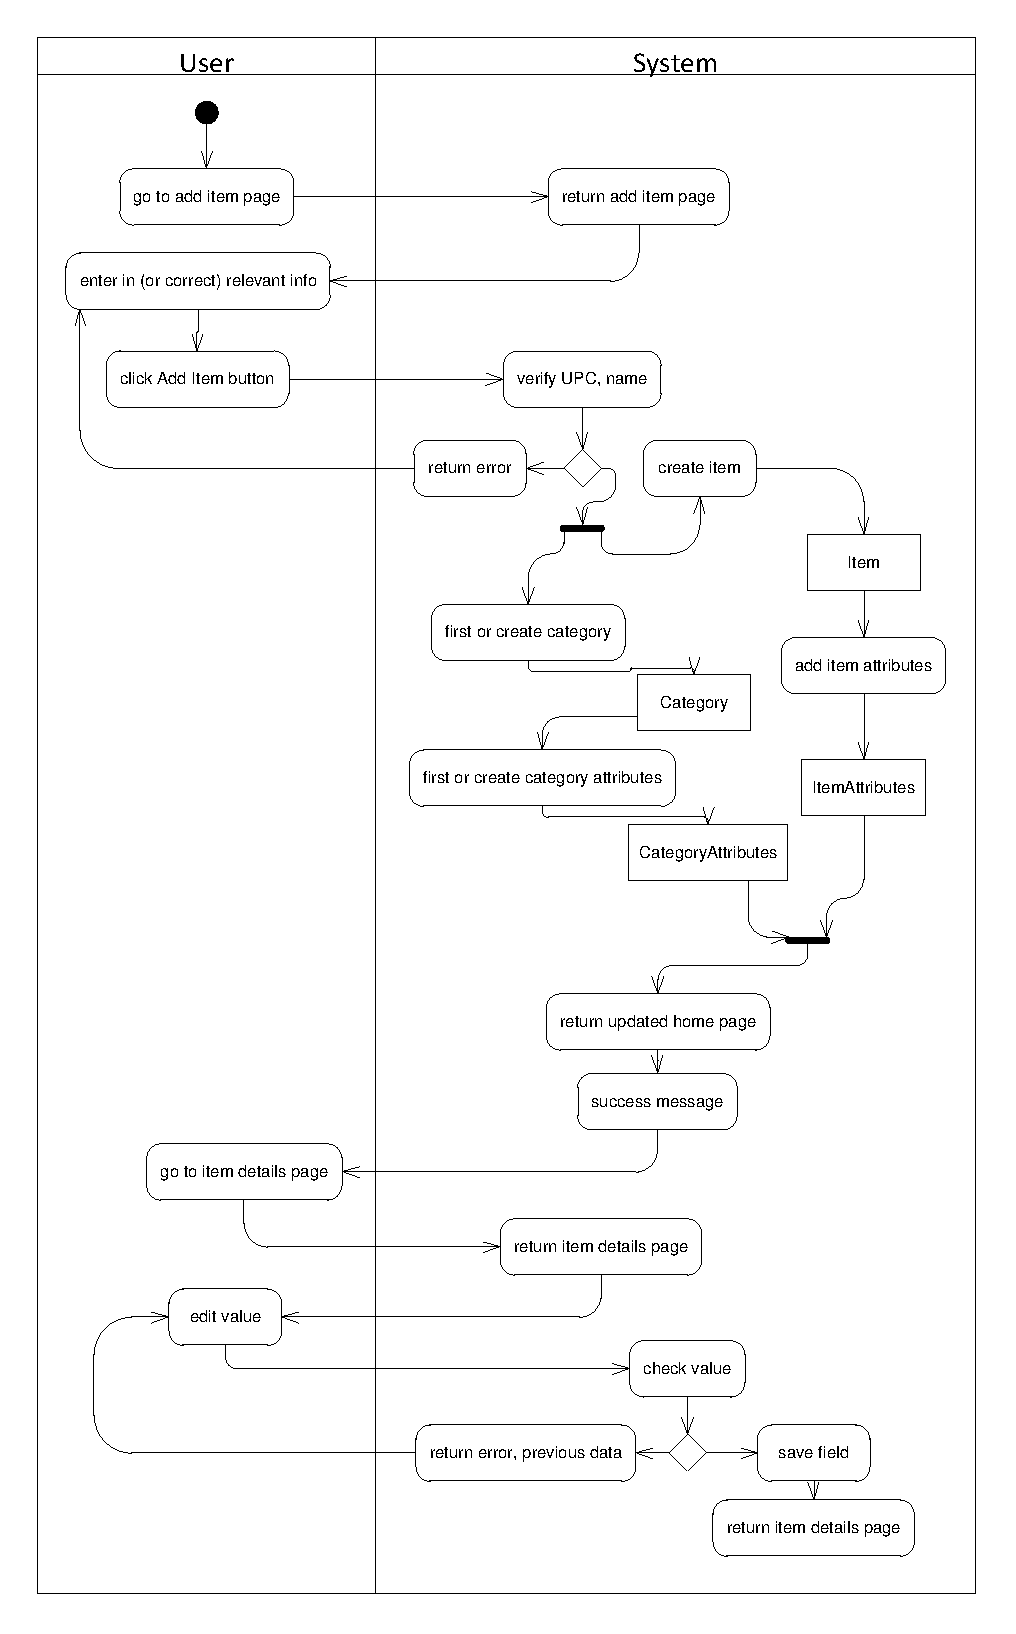
\includegraphics[keepaspectratio, width=5in]{activity_diagram.pdf}\\

\section{GRASP Principles}
\subsection{Creator}
The creator principle states that the class that creates or instantiates a new instance of a class should be one which contains, records, uses, or has the initializing data for that class. The AddItemController class would be the first class to have the necessary knowledge to create a new item object. Because of this, we choose to make this class responsible for creating a new item and adding it to the database.\\
\subsection{Controller}
For our project we have several user interface pages that each have a distinct purpose. The user will interact differently with each of these pages. In order to coordinate the system operations required by these pages, a controller is needed. As each interface is specific to a use case, our system will use a series of use case controllers. We will create them using the Sinatra framework. Each controller would be in charge of a small set of Sinatra routes, allowing it to pass commands to the back end.\\
\subsection{Indirection}
Indirection is inherent in our system as we are using Sinatra and DataMapper to separate the different layers we have. Sinatra connects our front end to our back end. The different Sinatra routes take in information from the user and then direct information and commands to the back end. In our back end, we use DataMapper to connect our classes to the database. This keeps a layer of separation between the two, allowing the classes to not worry about how the data must be sent to the database, and simply concentrate on what data must be sent.\\
\subsection{Pure Fabrication}
Our system closely models real world objects, but there are still things we had to create in order to make the software work. Our controller classes are essential to the system; however, in our world we have no need to have something actively place an object's information in our memory.\\
\subsection{Protected Variations}
Placing an object in between two classes is a way to wrap a volatile class. Although there is nothing in our system we expect to change frequently, there are still places we have put this layer of protection in place. Using DataMapper is an example of this principle in our system. As all of our object classes must access the database, having a wrapper for it is very important. Should our client wish to change databases, one simple change to how the database is instantiated is all that is necessary. We do not have to change any code, since DataMapper is what creates the queries, not our classes.\\

\section{Gang of Four Patterns}
The current Personal Inventory Manager implementation has some room to grow. Although the current implementation of the Personal Inventory Manager does not include any patterns, with more time it could use several. \\
\subsection{Factory}
In our system, when the user goes to create an item, the code to do that is currently (at the time of this writing) in the same controller class that formats the data that is sent to the add item page. This design could be improved by adding an ItemFactory that could handle the complex task of creating an Item, as creating an Item of a new Category or with new Attribute fields would cause new Item, Category, and Attribute objects to be created, linked together appropriately, then each would be saved in the database. This complex creation responsibility is an obvious candidate for a Factory. \\
\subsection{Composite}
Our system has no way to handle batch item operations; however, it would not be too difficult to imagine how a system like this might need to have the ability to batch process items, the ability to delete a category of items, as well as the items themselves, from the system. Another possibility would be the ability to export an item to a text file, as well as export all of the items in a set of search results to a text file. In examples such as these, it would make sense to have a SearchResults or Item Category class implement a shared interface with the item that would allow them to be treated the same. Then, no matter how many items are selected, they could all be printed or deleted simply, without needing to treat compositions of Items differently from a single Item.\\
\subsection{Fa\c{c}ade}
In our system there should be the ability to generate a report page. This page would have results calculated from data that could be poled from a myriad of different locations or objects. Because of its complexity and how deeply it is tied into so many different domain layer objects, it might make sense to have there be a façade to at least collect and compile the data that is going to be displayed on the page, and maybe even display it itself. This would effectively hide all of the data gathering and allow the UI controller to act simply as an interface between the web pages and the system, as opposed to forcing it to do all of the heavy lifting of generating the report data itself. \\

\section{Integration Tests}
This table shows which features have been implemented in our system by the end of Winter Quarter 2012.\\
\begin{tabular}{| l | c |}
\hline
\textbf{Feature}\label{feature} & \textbf{Complete}\\
\hline
\hline
Online UI & Yes \\
\hline
Add assets to the inventory & Yes \\
\hline
View all data associated with an item & Yes \\
\hline
Modify assets in the inventory & No \\
\hline
The system keeps track of attributes based on category & Yes \\
\hline
Use a UPC-A\label{upc} barcode as the unique identifier for each asset & Yes \\
\hline
Provide an updated list of recently-added assets & Yes \\
\hline
Generate reports of asset inventory & No \\
\hline
Sort search results based off of barcode, title, and modified / created timestamp & No \\
\hline
Basic search for items based on name or UPC & No \\
\hline
Advanced search for items based on all fields related to the item and its category & No \\
\hline
Basic and Advanced searches allow the user to include wildcards in the query & No \\
\hline
Basic and Advanced searches will search first by exact\label{exact} / wildcard\label{wild} match, then by fuzzy match\label{fuzzy} & No \\
\hline
REST API & No \\
\hline
\end{tabular}\label{rest}\\ \\ \\

\section{Acceptance Test Plan}
\label{test_case}

\paragraph{Test Case Syntax}
Each test case is divided into three sections:
\begin{itemize}
\item A ``Scenario Matrix'' section which describes each possible combination of flows (both basic and alternative) of a use case.
\item A ``Testing Matrix'' section which identifies distinct test cases defined by what conditions must be present in order to enact an expected result in response to the situation.
\item A ``Test Case to Scenario Matrix'' section which shows the correspondence between scenarios and test cases in order to help ensure completeness and traceability.
\end{itemize}

\subsection{Add an Item}
\textbf{NOTE:} Alternate Flow A0 will not be tested, since the server going offline is not an attribute of the system that can be measured.\label{flow}

\paragraph{Scenario Matrix}~\\ \\
\begin{tabular}{ c  c  c  c }
\hline
Scenario ID & Originating Flow & Alternate Flow & Next Alternate\label{scenario}\\
\hline
\hline
S0 & Basic &  & \\
\hline
S1 & Basic & A1 & \\
\hline
S2 & Basic & A2 & \\
\hline
S3 & Basic & A1 & A2\\
\hline
\end{tabular}\\
~\\
~\\
\paragraph{Testing Matrix}~\\ \\
\begin{tabular}{ p{0.8in}  p{0.7in}  p{0.7in}  p{3.3in} }
\hline
Test Case ID & Name Field & UPC Field & Expected Result\\
\hline
\hline
T0 & Present & Unique & The item is added successfully and the user is redirected to the main page with an updated Recent Changes list\\
\hline
T1 & Absent & Unique & The user is notified that a required field was omitted\\
\hline
T2 & Present & Absent & The user is notified that a required field was omitted\\
\hline
T3 & Absent & Absent & The user is notified that a required field was omitted\\
\hline
T4 & Present & Non-unique & The user is notified that the UPC is not unique\\
\hline
T5 & Absent & Non-unique & The user is notified that a required field was omitted and that the UPC is not unique\\
\hline
\end{tabular}\\
~\\
~\\
Present - a non-empty input\\
Absent - an empty input\\
Unique - a UPC code that is exclusive to the item\\
Non-unique - a UPC code that is no exclusive to the item
\paragraph{Test Case to Scenario Matrix}~\\ \\
\begin{tabular}{ | c || c | c | c | c | }
\hline
   & S0 & S1 & S2 & S3 \\
\hline
\hline
T0 & X  &    &    &    \\
\hline
T1 &    & X  &    &    \\
\hline
T2 &    & X  &    &    \\
\hline
T3 &    & X  &    &    \\
\hline
T4 &    &    & X  &    \\
\hline
T5 &    &    &    & X  \\
\hline
\end{tabular}

\subsection{Basic Search for an Item}
\textbf{NOTE:} Alternate Flow A1 will not be tested, since the server going offline is not an attribute of the system that can be measured.

\paragraph{Scenario Matrix}~\\ \\
\begin{tabular}{ c  c  c }
\hline
Scenario ID & Originating Flow & Alternate Flow\\
\hline
\hline
S4 & Basic &  \\
\hline
S5 & Basic & A0 \\
\hline
S6 & Basic & A2 \\
\hline
\end{tabular}\\
~\\
~\\
\paragraph{Testing Matrix}~\\ \\
\begin{tabular}{ p{0.8in}  p{0.75in}  p{0.5in}  p{3in} }
\hline
Test Case ID & Query Field & Matches & Expected Result\\
\hline
\hline
T6 & Present & Present & The results of the query are displayed on the page\\
\hline
T7 & Absent & & The user remains on the same page\\
\hline
T8 & Present & Absent & The text ``No results'' is displayed on the page\\
\hline
\end{tabular}\\
~\\
~\\
Present - a non-empty input\\
Absent - an empty input
\paragraph{Test Case to Scenario Matrix}~\\ \\
\begin{tabular}{ | c || c | c | c | }
\hline
   & S4 & S5 & S6 \\
\hline
\hline
T6 & X  &    &    \\
\hline
T7 &    & X  &    \\
\hline
T8 &    &    & X  \\
\hline
\end{tabular}


\subsection{Advanced Search for an Item}
\textbf{NOTE:} Alternate Flow A1 will not be tested, since the server going offline is not an attribute of the system that can be measured.

\paragraph{Scenario Matrix}~\\ \\
\begin{tabular}{ c  c  c  c }
\hline
Scenario ID & Originating Flow & Alternate Flow & Next Alternate \\
\hline
\hline
S7 & Basic &  & \\
\hline
S8 & Basic & A0 & \\
\hline
S9 & Basic & A0 & A2 \\
\hline
S10 & Basic & A0 & A3 \\
\hline
S11 & Basic & A3 &  \\
\hline
\end{tabular}\\
~\\
~\\
\paragraph{Testing Matrix}~\\ \\
\begin{tabular}{ p{0.8in}  p{0.5in} p{0.7in}  p{0.5in}  p{3in} }
\hline
Test Case ID & Category Field & Name/UPC Field & Matches & Expected Result\\
\hline
\hline
T9 & Present &  & Present & The results of the query are displayed on the page\\
\hline
T10 & Absent & Present & Present & The results of the query are displayed on the page\\
\hline
T11 & Absent & Absent &  & The user remains on the current page\\
\hline
T12 & Absent & Present & Absent & The text ``No results'' is displayed on the page\\
\hline
T13 & Present &  & Absent & The text ``No results'' is displayed on the page\\
\hline
\end{tabular}\\
~\\
~\\
Present - a non-empty input\\
Absent - an empty input
\paragraph{Test Case to Scenario Matrix}~\\ \\
\begin{tabular}{ | c || c | c | c | c | c | }
\hline
    & S7  & S8  & S9  & S10 & S11 \\
\hline
\hline
T9  &  X  &     &     &     &     \\
\hline
T10 &     &  X  &     &     &     \\
\hline
T11 &     &     &  X  &     &     \\
\hline
T12 &     &     &     &  X  &     \\
\hline
T13 &     &     &     &     &  X  \\
\hline
\end{tabular}

\subsection{Search Result Sorting}
\textbf{NOTE:} Alternate Flow A0 will not be tested, since the server going offline is not an attribute of the system that can be measured.
\paragraph{Scenario Matrix}~\\ \\
\begin{tabular}{ c  c }
\hline
Scenario ID & Originating Flow\\
\hline
\hline
S12 & Basic\\
\hline
\end{tabular}\\
~\\
~\\
\paragraph{Testing Matrix}~\\ \\
\begin{tabular}{ p{0.8in}  p{1.1in}  p{3.6in} }
\hline
Test Case ID & Sort Type Field & Expected Result\\
\hline
\hline
T14 & Name & The search results are sorted by the Name field\\
\hline
T15 & UPC & The search results are sorted by the UPC field\\
\hline
T16 & Recently Created & The search results are sorted by the Recently Created field\\
\hline
T17 & Recently Modified & The search results are sorted by the Recently Modified field\\
\hline
\end{tabular}\\
~\\
~\\
Name - a required field that serves as a label; sorting for this field is alphanumeric (ascending or descending)\\
UPC - a required field that serves as an unique identifier; sorting for this field is numeric (ascending or descending)\\
Recently Created - an automatically generated field that denotes the timestamp of when an item was added; sorting for this field is based on date and time (ascending or descending)\\
Recently Modified - an automatically generated field that denotes the timestamp of when an item was added or changed; sorting for this field is based on date and time (ascending or descending)
\paragraph{Test Case to Scenario Matrix}~\\ \\
\begin{tabular}{ | c || c | }
\hline
    & S12 \\
\hline
\hline
T14 &  X  \\
\hline
T15 &  X  \\
\hline
T16 &  X  \\
\hline
T17 &  X  \\
\hline
\end{tabular}

\subsection{View Details of an Item}
\textbf{NOTE:} Alternate Flow A0 will not be tested, since the server going offline is not an attribute of the system that can be measured.

\paragraph{Scenario Matrix}~\\ \\
\begin{tabular}{ c  c }
\hline
Scenario ID & Originating Flow\\
\hline
\hline
S13 & Basic\\
\hline
\end{tabular}\\
~\\
~\\
\paragraph{Testing Matrix}~\\ \\
\begin{tabular}{ p{0.8in}  p{3.4in} }
\hline
Test Case ID & Expected Result\\
\hline
\hline
T18 & The user is taken to a page showing all of the item details\\
\hline
\end{tabular}\\
~\\
~\\
\paragraph{Test Case to Scenario Matrix}~\\ \\
\begin{tabular}{ | c || c | }
\hline
    & S13 \\
\hline
\hline
T18 &  X  \\
\hline
\end{tabular}

\subsection{Edit Details of an Item}
\textbf{NOTE:} Alternate Flow A0 will not be tested, since the server going offline is not an attribute of the system that can be measured.
\paragraph{Scenario Matrix}~\\ \\
\begin{tabular}{ c  c  c }
\hline
Scenario ID & Originating Flow & Alternate Flow\\
\hline
\hline
S14 & Basic & \\
\hline
S15 & Basic & A1\\
\hline
\end{tabular}\\
~\\
~\\
\paragraph{Testing Matrix}~\\ \\
\begin{tabular}{ p{0.8in}  p{0.9in}  p{0.9in}  p{2.8in}}
\hline
Test Case ID & Name Field & UPC Field & Expected Result\\
\hline
\hline
T19 & Unchanged & Unchanged & The user is shown the item details page with the modified information\\
\hline
T20 & Valid Change & Unchanged & The user is shown the item details page with the modified information\\
\hline
T21 & Unchanged & Valid Change & The user is shown the item details page with the modified information\\
\hline
T22 & Valid Change & Valid Change & The user is shown the item details page with the modified information\\
\hline
T23 & Invalid Change & Unchanged & A pop-up with `Invalid Information' is shown\\
\hline
T24 & Invalid Change & Valid Change & A pop-up with `Invalid Information' is shown\\
\hline
T25 & Invalid Change & Invalid Change & A pop-up with `Invalid Information' is shown\\
\hline
T26 & Unchanged & Invalid Change & A pop-up with `Invalid Information' is shown\\
\hline
T27 & Valid Change & Invalid Change & A pop-up with `Invalid Information' is shown\\
\hline
\end{tabular}\\
~\\
~\\
Unchanged - the field was not modified\\
Valid Change (relative to Name Field) - the field was modified to be non-empty\\
Valid Change (relative to UPC Field) - the field was modified to be non-empty and unique\\
Invalid Change (relative to Name Field) - the field was modified to be empty\\
Invalid Change (relative to UPC Field) - the field was modified to be empty or non-unique
\paragraph{Test Case to Scenario Matrix}~\\ \\
\begin{tabular}{ | c || c | c | }
\hline
    & S14 & S15 \\
\hline
\hline
T19 &  X  &     \\
\hline
T20 &  X  &     \\
\hline
T21 &  X  &     \\
\hline
T22 &  X  &     \\
\hline
T23 &     &  X  \\
\hline
T24 &     &  X  \\
\hline
T25 &     &  X  \\
\hline
T26 &     &  X  \\
\hline
T27 &     &  X  \\
\hline
\end{tabular}

\subsection{Generate Inventory Report}
\textbf{NOTE:} Alternate Flow A0 will not be tested, since the server going offline is not an attribute of the system that can be measured.

\paragraph{Scenario Matrix}~\\ \\
\begin{tabular}{ c  c }
\hline
Scenario ID & Originating Flow \\
\hline
\hline
S16 & Basic \\
\hline
\end{tabular}\\
~\\
~\\
\paragraph{Testing Matrix}~\\ \\
\begin{tabular}{ p{0.8in}  p{2.2in} }
\hline
Test Case ID & Expected Result\\
\hline
\hline
T28 & The report is displayed on the page\\
\hline
\end{tabular}\\
~\\
~\\
\paragraph{Test Case to Scenario Matrix}~\\ \\
\begin{tabular}{ | c || c | }
\hline
    & S16  \\
\hline
\hline
T28 &  X  \\
\hline
\end{tabular}


\section{Who done what}
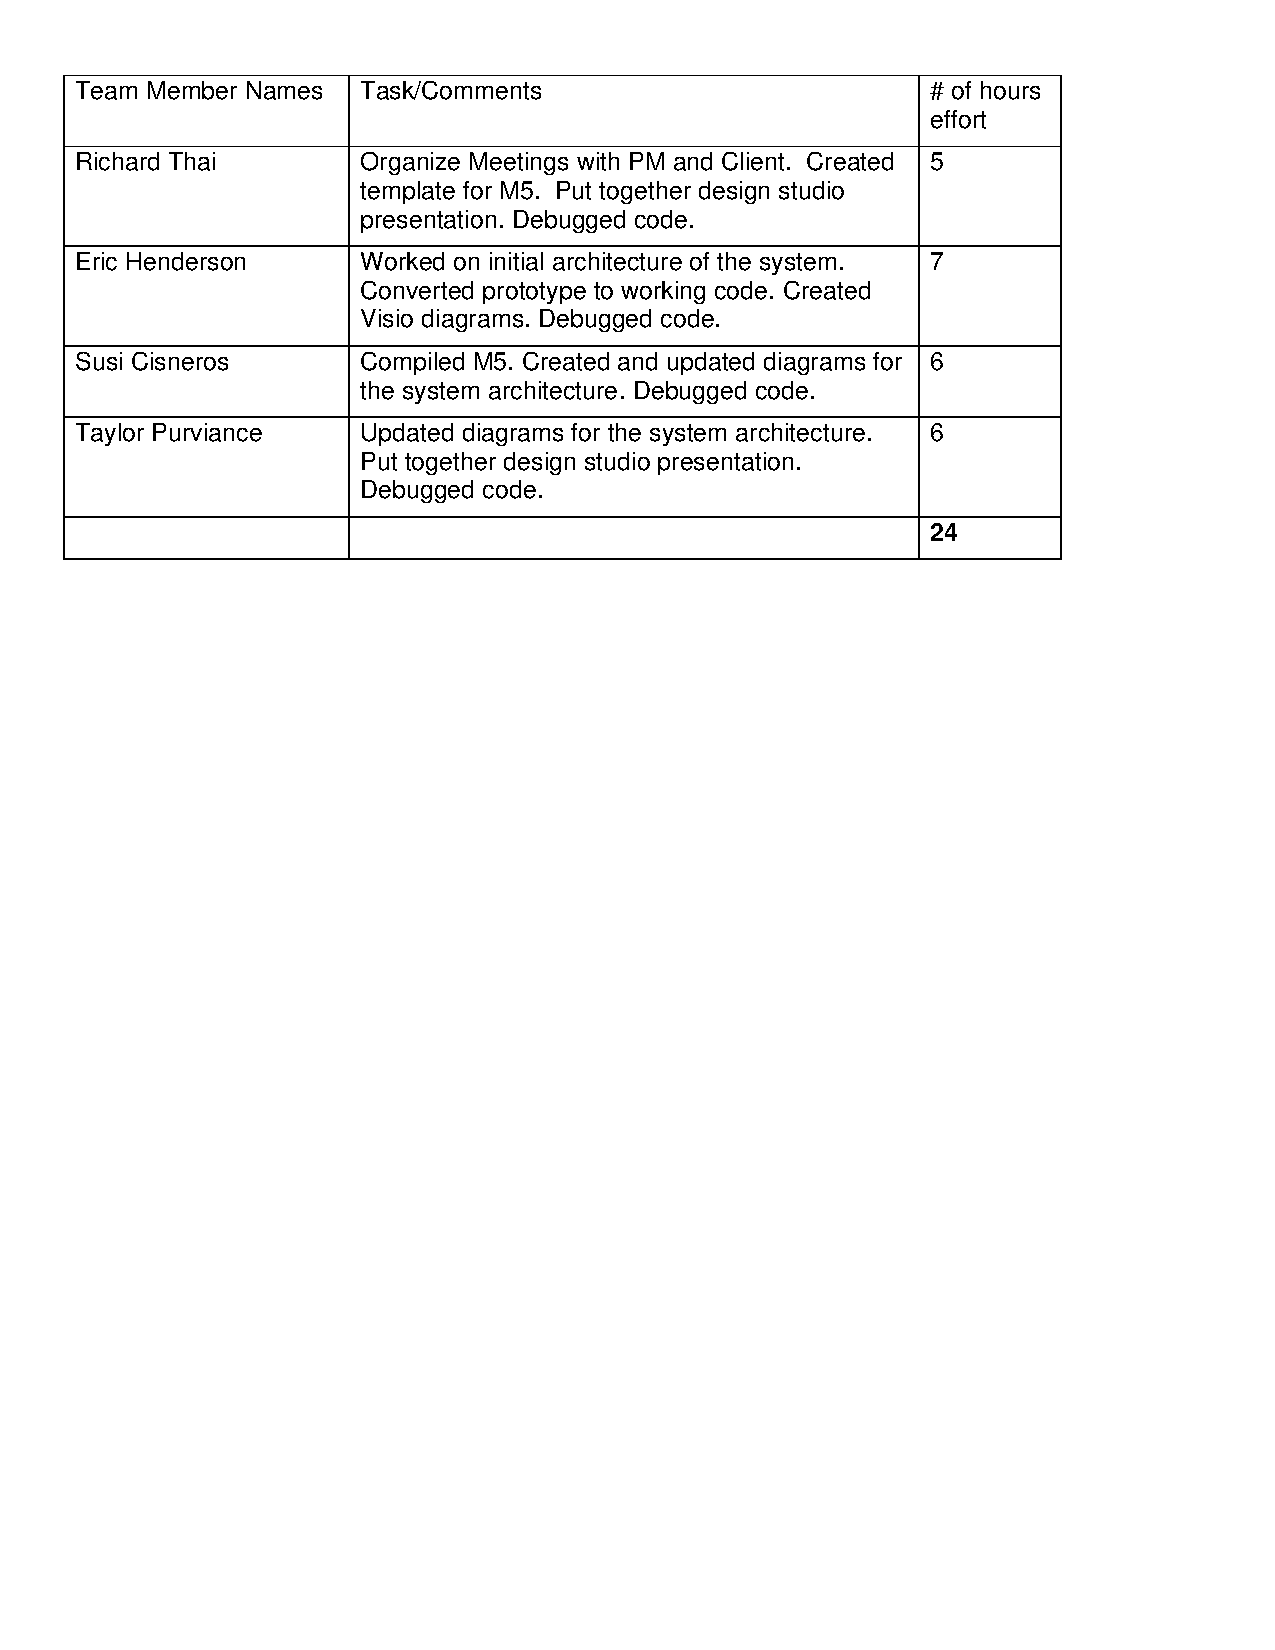
\includegraphics[keepaspectratio, width=6in]{wdwM5.pdf}\\

\section{Index and Glossary}
\textbf{Exact Match}: Valid search candidates are determined by strict equality with the search input(s) (\pageref{exact}).\\ \\
\textbf{Feature}: A system capability that fulfills a user need (\pageref{feature}).\\ \\
\textbf{Flow}: A particular series of ordered steps through a sequence of events in a use case (\pageref{flow}).\\ \\
\textbf{Fuzzy Match}: Valid search candidates are determined based on similarity to the original search input(s) (\pageref{fuzzy}).\\ \\
\textbf{REST}: Stands for ``Representational state transfer;'' is a style software architecture often used in servers for simplicity and scalability. Amongst other aspects of REST, it is stateless. This means each request sent from the client of the server that uses REST to the server does not require any information from any previous requests. All information required to fulfill the request must be sent with the request (\pageref{rest}).\\ \\
\textbf{Scenario}: A possible permutation of a set of flows that lead from one flow to another (\pageref{scenario}).\\ \\
\textbf{Test Case}: Specifies what the expected result of a series of actions will have in a system (\pageref{test_case}).\\ \\
\textbf{Universal Product Code (UPC)}: a specific kind of barcode assign uniquely to each item in the server (\pageref{upc}).\\ \\
\textbf{Wildcard Matching}: Valid search candidates are determined based on adherence to the user's given search pattern (\pageref{wild}).\\ \\

\section{References}
\hangindent=1.4cm
\textbf{(1)} Leffingwell, Dean, and Don Widrig.
\emph{Managing Software Requirements: a Use Case Approach}.
Addison-Wesley, Boston,
2nd Edition,
2003.\\

\noindent\hangindent=1.4cm
\textbf{(2)} ``Ruby 1.9.2''
\emph{Download Ruby.} Ruby. Web.  6 October 2011. \\

\noindent\hangindent=1.4cm
\textbf{(3)} ``Sinatra 1.3.0''
\emph{Sinatra: Documentation.} Sinatra. Web.  6 October 2011.\\

\noindent\hangindent=1.4cm
\textbf{(4)} ``Ubuntu 11.04''
\emph{Download Ubuntu.} Ubuntu. Web.  6 October 2011.\\

\noindent\hangindent=1.4cm
\textbf{(5)} ``SQLite 3.7.8''
\emph{SQLite Download Page.} SQLite. Web.  6 October 2011.\\

\noindent\hangindent=1.4cm
\textbf{(6)} ``Cucumber 1.1.0''
\emph{cucumber/cucumber.} Cucumber. Web.  6 October 2011.\\

\noindent\hangindent=1.4cm
\textbf{(7)} ``RSpec 2.6.0''
\emph{RSpec Documentation.} Relish. Web.  6 October 2011.\\

\noindent\hangindent=1.4cm
\textbf{(8)} ``DataMapper 1.1.0''
\emph{DataMapper - Documentation.} DataMapper. Web.  6 October 2011.\\

\noindent\hangindent=1.4cm
\textbf{(9)} ``Google Chrome 14.0.8'' 
\emph{About Google Chrome.} Google. Web.  7 October 2011.\\

\noindent\hangindent=1.4cm
\textbf{(10)} ``Firefox 7.0.1''
\emph{Mozilla Firefox Web Browser - Free Download.} Mozilla. Web.  7 October 2011.\\

\noindent\hangindent=1.4cm
\textbf{(11)} ``Apache 2.2''
\emph{Apache HTTP Server Version 2.2 Documentation - Apache HTTP Server.} Apache. Web.  7 October 2011.\\

\noindent\hangindent=1.4cm
\textbf{(12)} ``BSD''
\emph{The FreeBSD Copyright.} The FreeBSD Project. Web. 18 October 2011.\\

\noindent\hangindent=1.4cm
\textbf{(13)} ``GitHub''
\emph{GitHub - Social Coding.} GitHub, Inc. Web. 28 October 2011.\\

\noindent\hangindent=1.4cm
\textbf{(14)} ``The Unofficial Ruby Usage Guide'' \emph{The Unofficial Ruby Usage Guide.} Caliban. 28 October 2011.\\

\end{document}